% ==============================================================================
%
%                                    DVG303
%                  Objektorienterad design och programmering
%                                Laboration #2
%
% Author:   Jonas Sjöberg
%           Högskolan i Gävle
%           tel12jsg@student.hig.se
%           https://github.com/jonasjberg
%
% License:  Creative Commons Attribution-NonCommercial-ShareAlike 4.0
%           International.  See LICENSE.md for full licensing information.
% ==============================================================================

\documentclass[11pt,a4paper]{article}
\usepackage[utf8]{inputenc}
\inputencoding{utf8}
\usepackage[swedish]{babel}
\usepackage[swedish]{isodate}
\usepackage[T1]{fontenc}
\usepackage{lmodern}
\usepackage{fullpage}

\usepackage{textcomp}
\usepackage{url}
\usepackage{graphicx}

\usepackage{minted}
\usemintedstyle{bw}

\usepackage{verbatim}
\usepackage{fancyvrb}
\usepackage{listings}

\usepackage[pdfusetitle,bookmarks=true,
 bookmarksnumbered=true,bookmarksopen=false,
 breaklinks=false,pdfborder={0 0 0},backref=false,
 colorlinks=false]{hyperref}

\newmintedfile[javacode]{java}{
%bgcolor=mintedbackground,
%fontfamily=tt,
fontsize=\footnotesize,
linenos=true,
numberblanklines=true,
numbersep=12pt,
numbersep=5pt,
frame=lines,
framesep=2mm,
funcnamehighlighting=true,
tabsize=4,
obeytabs=false,
mathescape=false
samepage=false,
showspaces=false,
showtabs =false,
texcl=false,
}

\title{DVG303 \\ Objektorienterad design och programmering \\ Laboration 2}

\author{\\
  Jonas Sjöberg\\
  860224\\
  Högskolan i Gävle\\
  \texttt{tel12jsg@tudent.hig.se}\\
  \texttt{https://github.com/jonasjberg}\\
}


\date{}

\begin{document}
    \maketitle

    \begin{center}
    \begin{tabular}{l r}
        Datum: & \isodate \today \par \\
        Kursansvarig lärare: & Atique Ullah
    \end{tabular}
    \end{center}

    \medskip

    \begin{abstract}
        Laborationsrapport för
        \emph{DVG303 -- Objektorienterad design och programmering},
        Högskolan i Gävle, Höstterminen 2015.
    \end{abstract}

    \newpage
    \setcounter{tocdepth}{3}
    \tableofcontents
    \listoffigures
    \newpage

    %% ==============================================================================
%                                    DVG303
%                  Objektorienterad Design och Programmering
%                                Laboration #2
%
% Author:   Jonas Sjöberg
%           Högskolan i Gävle
%           tel12jsg@student.hig.se
%           https://github.com/jonasjberg
%
% License:  Creative Commons Attribution-NonCommercial-ShareAlike 4.0
%           International.  See LICENSE.md for full licensing information.
% ==============================================================================

\section*{Introduktion}\label{sec:intro}
\addcontentsline{toc}{section}{Introduktion}

\subsection*{Övergripande beskrivning}\label{sec:beskrivning}
\addcontentsline{toc}{subsection}{Övergripande beskrivning}
Det här är den andra av tre laborationer i objektorienterad design och
programmering. Ett fullständigt program kommer att utvecklas under
laborationerna. Processen kommer att innehålla många element av professionell
mjukvaruutveckling; design, dokumentation, revisionskontroll, etc., och syftar
till att utveckla praktiska färdigheter i mjukvaruutveckling.

\subsection*{Uppgifter}
\addcontentsline{toc}{subsection}{Uppgifter}
Instruktionerna är till viss del kopierade från källfilen
\texttt{oodp\_lab\_instruktioner\_ht15v4.pdf}.

\subsection*{Arbetsmetod}
\addcontentsline{toc}{subsection}{Arbetsmetod}
\begin{itemize}
    \item Koden skrivs i utvecklingsmiljön \texttt{Intellij IDEA} under
          \texttt{Linux 3.19.0-28-generic} och kompileras samt exekveras med 
          följande \texttt{Java}-version:
\begin{verbatim}
> $ java -version
java version "1.7.0_79"
OpenJDK Runtime Environment (IcedTea 2.5.6) (7u79-2.5.6-0ubuntu1.15.04.1)
OpenJDK Server VM (build 24.79-b02, mixed mode)
\end{verbatim}

    \item Rapporten skrivs i \LaTeX\ med texteditorn \texttt{Vim} och kompileras
          till pdf med \texttt{latexmk}.  \par Diagram och figurer skrivs i
          \texttt{PlantUML}-format och renderas med \texttt{Graphviz}. 
          Resultatet förhandsgranskas i realtid med hjälp av plugins i 
          \texttt{Intellij IDEA}.

    \item För revisionskontroll används \texttt{Git}.

    \item Analys av program under exekvering sker med hjälp av 
          \texttt{JIVE} -- Java Interactive Visualization Environment.
          \footnote{\url{http://www.cse.buffalo.edu/jive/}}

\end{itemize}

UML-diagram och dokumentation uppdateras löpande parallellt med källkoden.
Förändringar i källkoden har kommit att följa uppdaterade diagram likväl som
diagrammen har behövt uppdateras för att reflektera förändrad källkod eller
funktionalitet.
\par Varje uppgift finns representerad som en separat utvecklingsgren
(\emph{branch}) i \texttt{Git}. På så vis kan varje uppgift utvecklas oberoende
utan redundans och filduplicering. Det är också mycket enkelt att propagera
förändringar mellan grenar och individuella \emph{commits} med hjälp av
ändamålsriktiga ``diff''-verktyg. Ett sådant ingår i standarddistributioner av
\texttt{Git}, ett annant exempel är \texttt{Meld}.


\subsection*{Källkod}
\addcontentsline{toc}{subsection}{Källkod}
\par Källkod till programmet och rapporten finns att hämta på
\url{https://github.com/jonasjberg/DVG303_lab2}.
Hämta hem repon genom att exekvera följande från kommandoraden:
\begin{verbatim}
> $ git clone git@github.com:jonasjberg/DVG303_lab2.git
\end{verbatim}


    % ==============================================================================
%
%                                    DVG303
%                  Objektorienterad design och programmering
%                                Laboration #2
%
% Author:   Jonas Sjöberg
%           Högskolan i Gävle
%           tel12jsg@student.hig.se
%           https://github.com/jonasjberg
%
% License:  Creative Commons Attribution-NonCommercial-ShareAlike 4.0
%           International.  See LICENSE.md for full licensing information.
% ==============================================================================

\section{Uppgift 1}\label{sec:uppg01}

\subsection{Instruktioner}
\begin{Verbatim}[fontsize=\small]
Skriv ett program där man ska skriva in ett antal heltal. Hur många tal ska den
som kör programmet själv bestämma, dock max 30. Heltalen ska lagras i en array.

Programmet ska sedan beräkna summan av talen, beräkna talens medelvärde
(exakta), ta reda på vilket av talen som är störst och minst. Exempel på hur
utskriften kan se ut (inmatning från tangentbordet = *fetstil*):

Hur många tal vill du mata in (max 30)? *5*
*4*
*5*
*3*
*7*
*6*
Summa: 25
Medelvärde: 5.0
Minsta värde: 3
Största värde: 7
\end{Verbatim}


\subsection{Källkod}
\subsubsection{Lab4Uppg01.java}
\javacode{src/Lab4Uppg01.java}
\caption{Lab4Uppg01.java}
\label{src:uppg01}

\subsubsection{UserInputFilter.java}
\javacode{src/UserInputFilter.java}
\caption{UserInputFilter.java}
\label{src:userinputfilter}


% Screenshots med Bash, terminalfönsterstorlek 90x40
\subsection{Skärmdump}
Se Figur~\ref{fig:uppg01-screenshot} för skärmdump på körning av koden i
Sektion~\ref{src:uppg01} och Sektion~\ref{src:userinputfilter}.

\begin{figure}[htbp]
\centering
\includegraphics[width=\linewidth]{img/01.png}
\caption{Körning av koden till Uppgift~\ref{sec:uppg01}}
\label{fig:uppg01-screenshot}
\end{figure}


    % ==============================================================================
%                                    DVG303
%                  Objektorienterad design och programmering
%                                Laboration #2
%
% Author:   Jonas Sjöberg
%           Högskolan i Gävle
%           tel12jsg@student.hig.se
%           https://github.com/jonasjberg
%
% License:  Creative Commons Attribution-NonCommercial-ShareAlike 4.0
%           International.  See LICENSE.md for full licensing information.
% ==============================================================================

\section{Uppgift 2}\label{sec:uppg2}

\subsection{}\label{sec:uppg2a}
\subsubsection*{Frågeställning}
Ändra modellklasserna från laboration 1 så att de implementerar interfacen
ifall det passar.

\subsubsection*{Lösning}
Den enklaste figur-klassen \texttt{Figure} implementerar interfacet
\texttt{Movable}.  Underklasserna \texttt{Point}, \texttt{Circle} och
\texttt{Ellipse} implementerar sedan \texttt{Scalable} och \texttt{Rotatable}
beroende på vad som är lämpligt för respektive klass.

\begin{itemize}
\item \texttt{Point} behöver varken roteras eller skalas och implementerar
      indirekt \texttt{Movable} genom superklassen \texttt{Figure}.
\item \texttt{Circle} kan skalas men behöver inte roteras och implementerar
      följdaktligen \texttt{Movable} (ärvs från superklassen) och 
      \texttt{Scalable}.
\item \texttt{Ellipse} kan både skalas och roteras och implementerar
      \texttt{Movable} (ärvs från superklassen), \texttt{Rotatable} och 
      \texttt{Scalable}.
\end{itemize}

Jag inser nu att arvshierarkin är onödigt komplex, det finns ingen större vits
med att ha två separata arvsträd av figurtyper, \texttt{SimpleFigure} och
\texttt{Figure}. Men vid det här laget finns inte tid för någon
omstrukturering.


\subsection{}\label{sec:uppg2b}
\subsubsection*{Frågeställning}
Varje klass i dataskiktet som kan instansieras ska kompletteras med en metod
toString (för mer information se PDF-filen Chapter3.pdf, ’Item 10: Always
override toString’).

\subsubsection*{Lösning}
Se bifogad källkod. Lösningen använder \texttt{StringBuilder} för att
konkatenera resultatet från superklassens \texttt{toString}-metod med klassens
egna data.


\subsection{}\label{sec:uppg2c}
\subsubsection*{Frågeställning}
Diskutera: Varför används typer som \texttt{List<FigureType>} i FigureHandler?
Kan man inte använda bara List? Eller en array?


\subsubsection*{Lösning}
Användningen av en \texttt{List} framför en vanlig array motiveras med att en
array inte kan ändra storlek dynamiskt. Storleken definieras vid skapande av
arrayen och är därefter fixerad. En \texttt{List} har flera användbara
funktioner som saknas för arrays. Genom att skriva något i stil med
\texttt{List<Figure>} specifieras vilken typ av objekt listan kan innehålla.
Det fungerar som en slags felkontroll där kompilatorn ger varningar om ett
inkompatibelt objekt stoppas in.



    % ==============================================================================
%                                    DVG303
%                  Objektorienterad design och programmering
%                                Laboration #2
%
% Author:   Jonas Sjöberg
%           Högskolan i Gävle
%           tel12jsg@student.hig.se
%           https://github.com/jonasjberg
%
% License:  Creative Commons Attribution-NonCommercial-ShareAlike 4.0
%           International.  See LICENSE.md for full licensing information.
% ==============================================================================

\section{Uppgift 3}\label{sec:uppg3}

\subsection{}\label{sec:uppg3a}
\subsubsection*{Frågeställning}
När metoden \texttt{createPoint} anropas på ett objekt av typen
\texttt{FigureHandler}, så måste det skickas ett antal meddelanden mellan olika
objekt. Visa meddelanden med hjälp av ett sekvensdiagram!

\subsubsection*{Lösning}
Programexekveringen analyserades med \texttt{JIVE} -- Java Interactive
Visualization Environment. \footnote{\url{http://www.cse.buffalo.edu/jive/}}

\texttt{JIVE} installeras som plugin i \texttt{Eclipse Mars} version 4.5.0 och
körs i ett interaktivt debug-``perspective''. Programmet kan generera olika
modeller av ett program;

\begin{enumerate}
\item Contour Model.
\item Object Diagram.
\item Sequence Model.
\item Sequence Diagram.
\item Event Log.
\end{enumerate}

En särskild klass vid namn \texttt{FigureHandlerTest} används vid körning
av \texttt{JIVE}, som kan presentera resultatet på olika sätt. Jag valde att
exportera som \texttt{csv}-textfil samt \texttt{png}-bild.

Sekvensdiagram för programmet \texttt{FigureHandlerTest} återfinns i
Figur~\ref{fig:sekv-point}, Figur~\ref{fig:sekv-line},
Figur~\ref{fig:sekv-rect} och Figur~\ref{fig:sekv-all}.
Resultatet av testerna är finns också bifogade i katalogen \texttt{diagram}.

% JIVE: Dynamic Analysis for Java
% Overview, Architecture, and Implementation
% Demian Lessa
% Computer Science and Engineering
% State University of New York, Buffalo
% http://www.cse.buffalo.edu/jive/presentations/cse505-10-12-01.pdf

% Jive
% Tool Overview
% April 07 :: Spring 2010
% Demian Lessa <dlessa@buffalo.edu>
% http://www.cse.buffalo.edu/jive/presentations/cse605-10-04-07a.pdf

%\begin{sidewaysfigure}[ht]
\begin{figure}[ht]
\centering
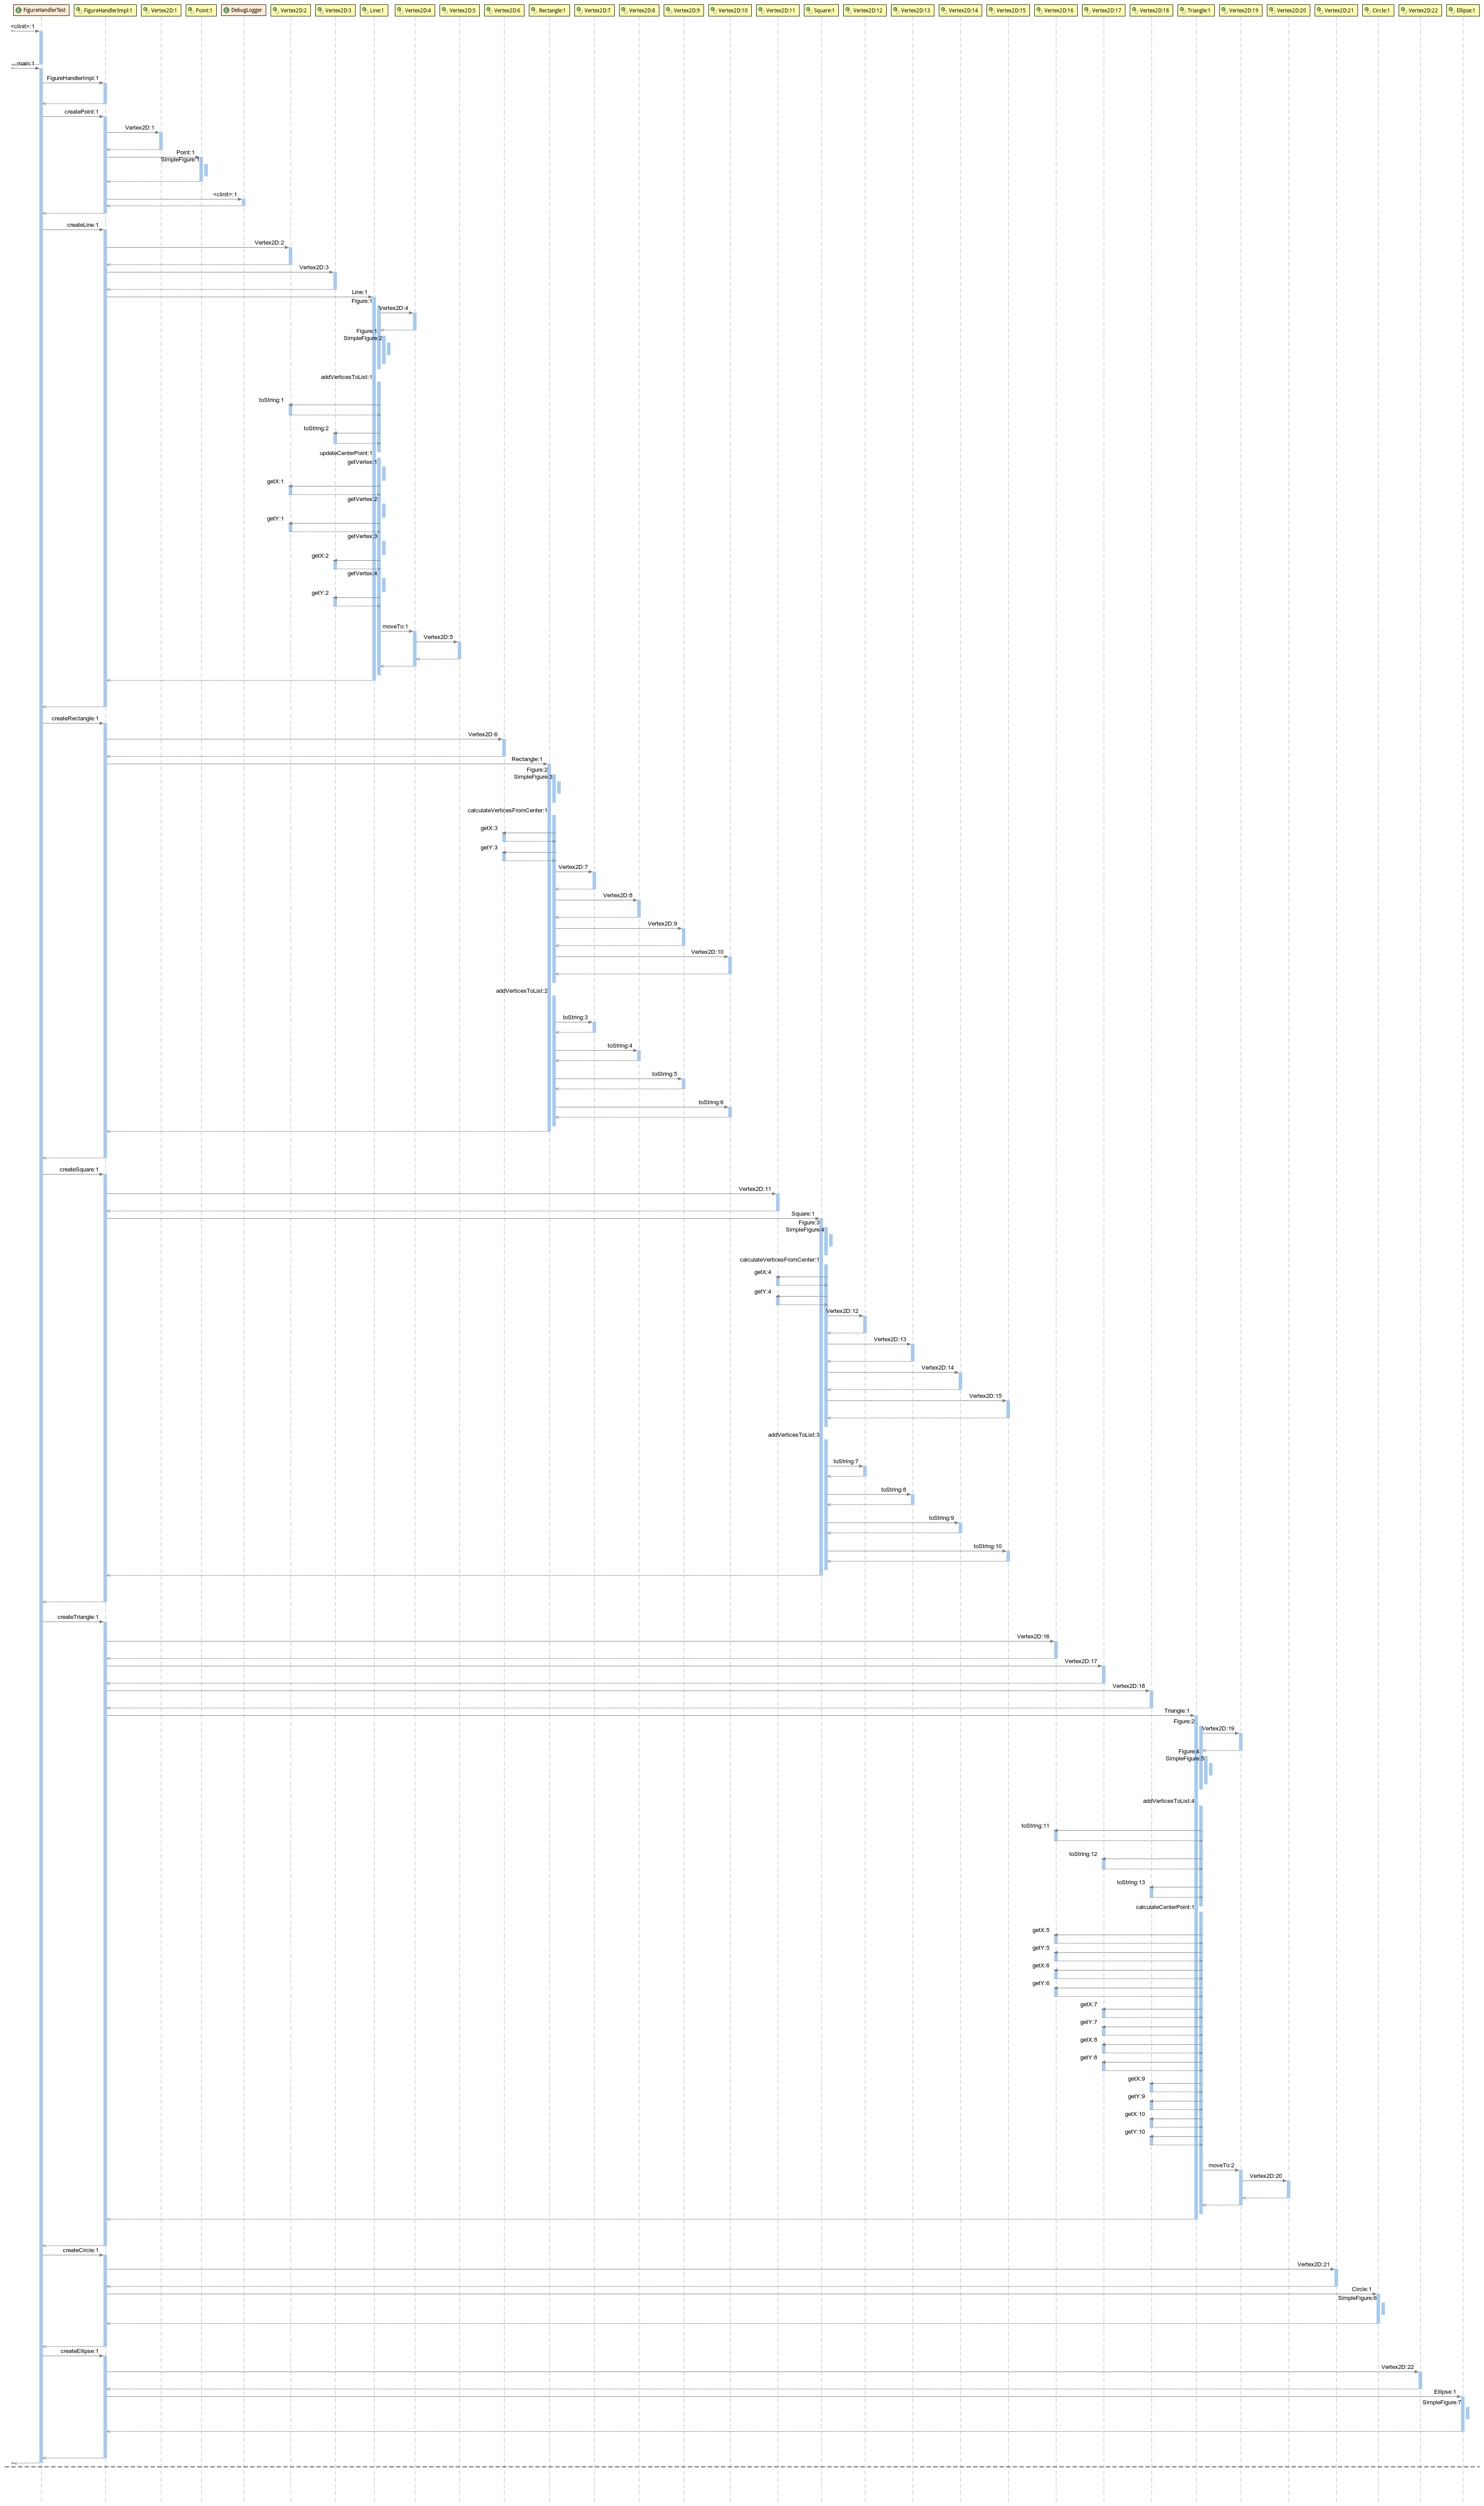
\includegraphics[width=0.9\linewidth]{diagram/figureHandlerTest_All_Sequence-Diagram.png}
\caption{Uppgift~3\ref{sec:uppg1b}: Sekvensdiagram för test av alla figurer.
\\ (\texttt{diagram/figureHandlerTest\_All\_Sequence-Diagram.png})}
\label{fig:sekv-all}
%\end{sidewaysfigure}
\end{figure}

\begin{figure}[ht]
\centering
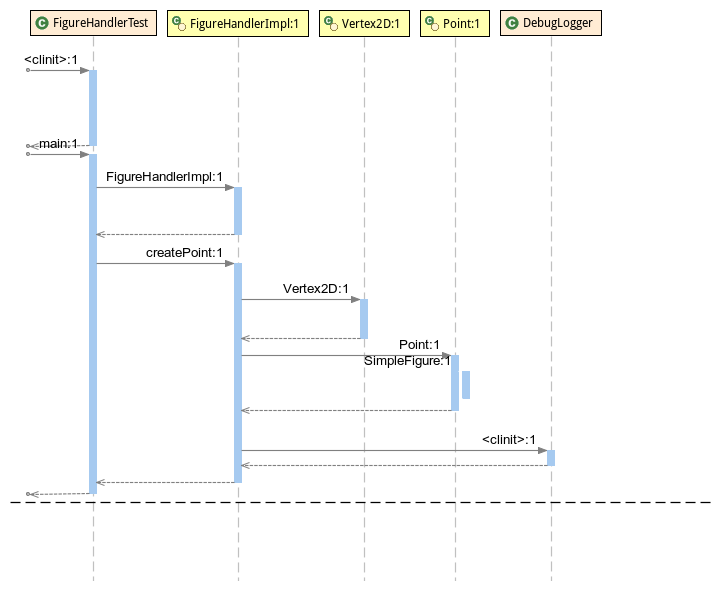
\includegraphics[width=\linewidth]{diagram/figureHandlerTest_Point_Sequence-Diagram.png}
\caption{Uppgift~3\ref{sec:uppg1b}: Sekvensdiagram för \texttt{Point}.
\\ (\texttt{diagram/figureHandlerTest\_Point\_Sequence-Diagram.png})}
\label{fig:sekv-point}
\end{figure}

\begin{figure}[ht]
\centering
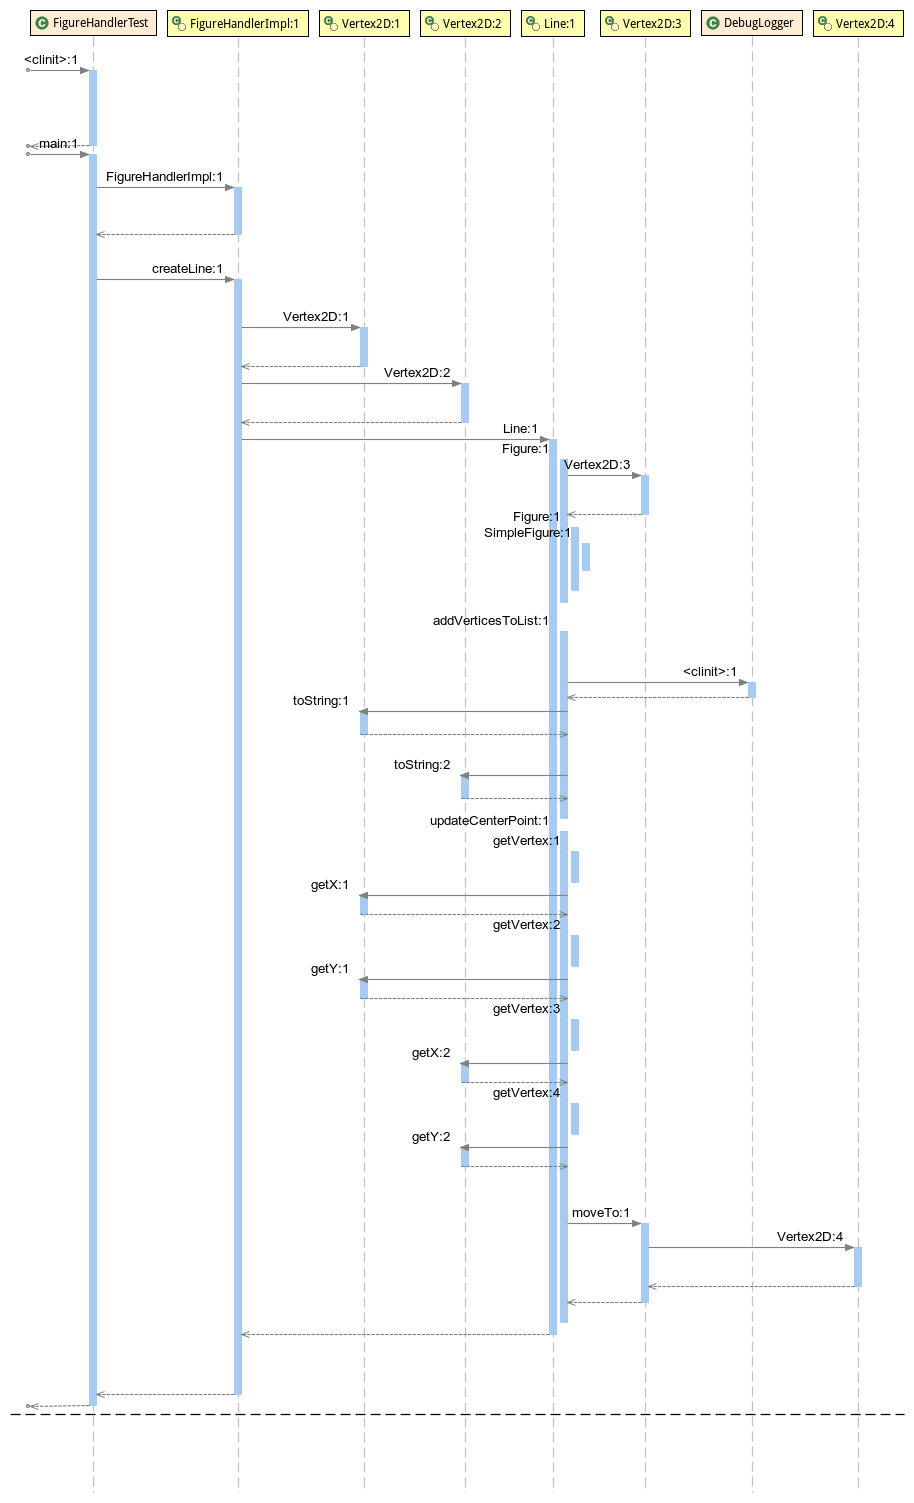
\includegraphics[width=0.8\linewidth]{diagram/figureHandlerTest_Line_Sequence-Diagram.png}
\caption{Uppgift~3\ref{sec:uppg1b}: Sekvensdiagram för \texttt{Line}.
\\ (\texttt{diagram/figureHandlerTest\_Line\_Sequence-Diagram.png})}
\label{fig:sekv-line}
\end{figure}

\begin{figure}[ht]
\centering
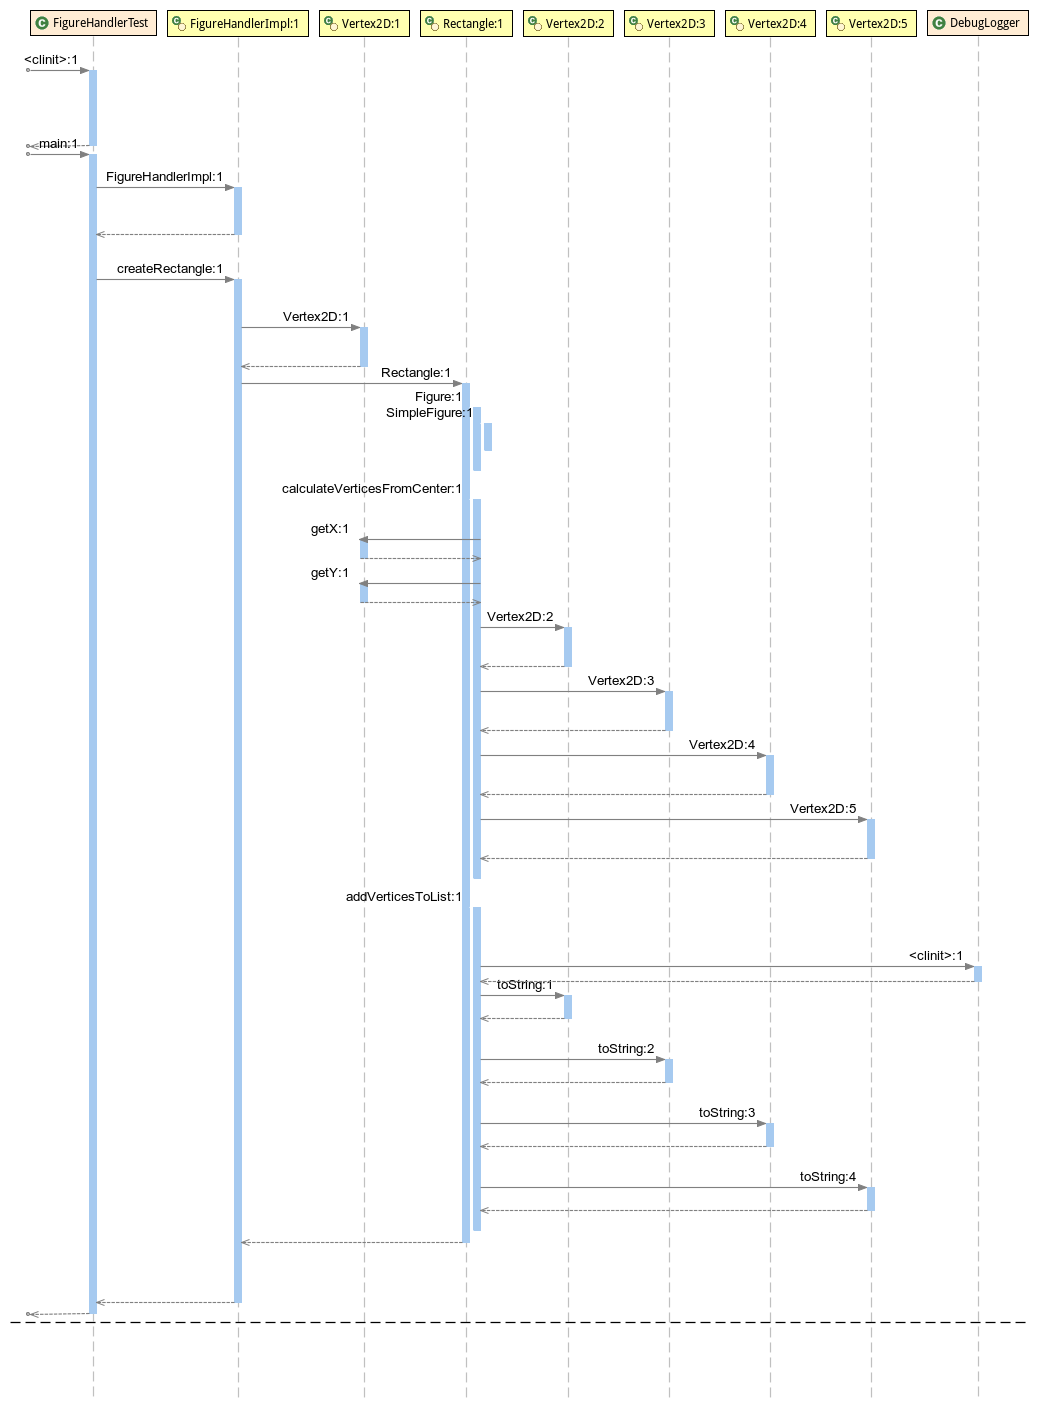
\includegraphics[width=\linewidth]{diagram/figureHandlerTest_Rectangle_Sequence-Diagram.png}
\caption{Uppgift~3\ref{sec:uppg1b}: Sekvensdiagram för \texttt{Rectangle}.
\\ (\texttt{diagram/figureHandlerTest\_Rectangle\_Sequence-Diagram.png})}
\label{fig:sekv-rect}
\end{figure}

\begin{sidewaysfigure}
%\begin{figure}[ht]
\centering
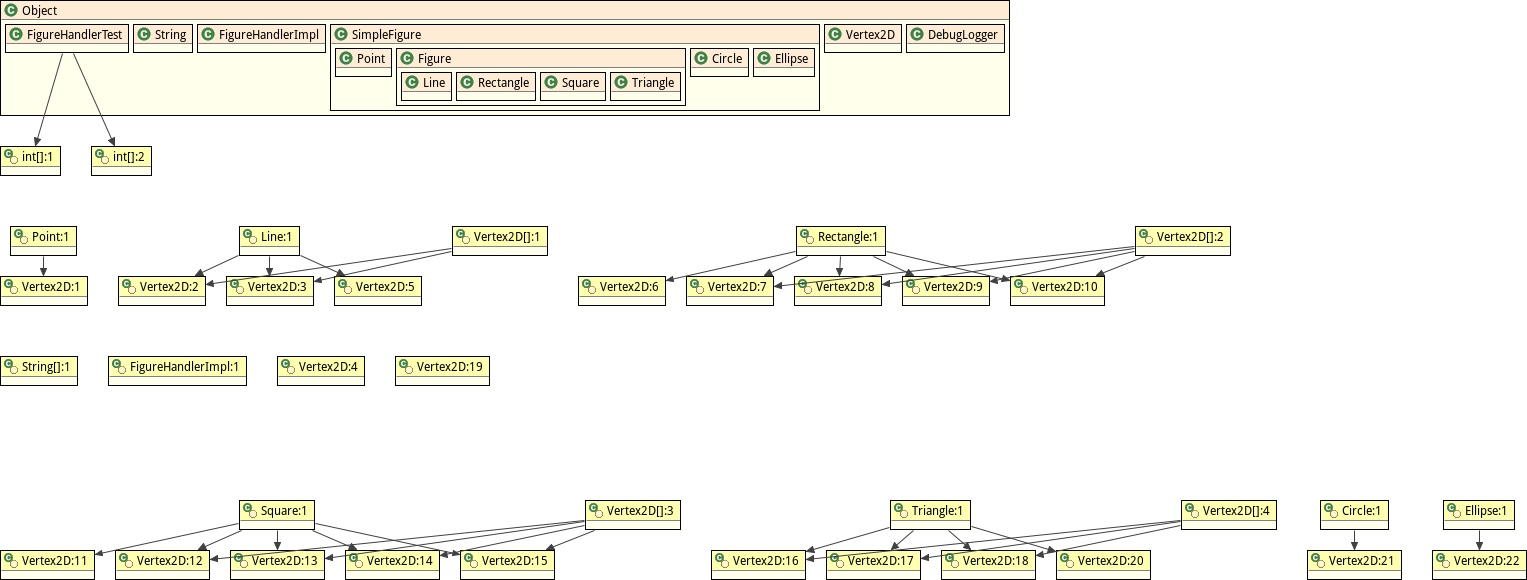
\includegraphics[width=\linewidth]{diagram/figureHandlerTest_All_Object-Diagram.png}
\caption{Uppgift~3\ref{sec:uppg1b}: Objektdiagram för test av alla figurer.
\\ (\texttt{diagram/figureHandlerTest\_All\_Object-Diagram.png})}
\label{fig:obj-all}
%\end{figure}
\end{sidewaysfigure}

\begin{figure}[ht]
\centering
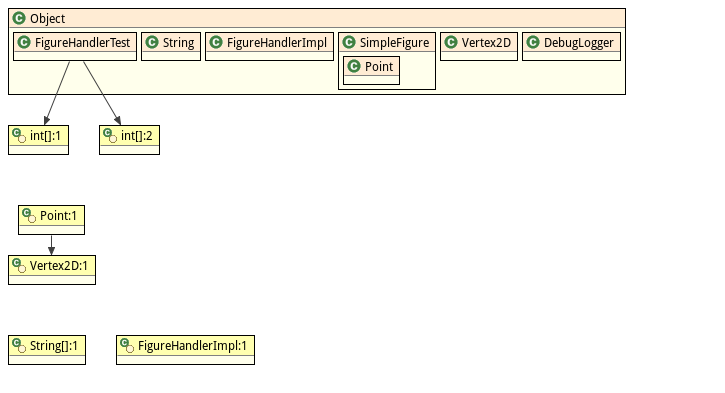
\includegraphics[width=\linewidth]{diagram/figureHandlerTest_Point_Object-Diagram.png}
\caption{Uppgift~3\ref{sec:uppg1b}: Objektdiagram för \texttt{Point}.
\\ (\texttt{diagram/figureHandlerTest\_Point\_Object-Diagram.png})}
\label{fig:obj-point}
\end{figure}

\begin{figure}[ht]
\centering
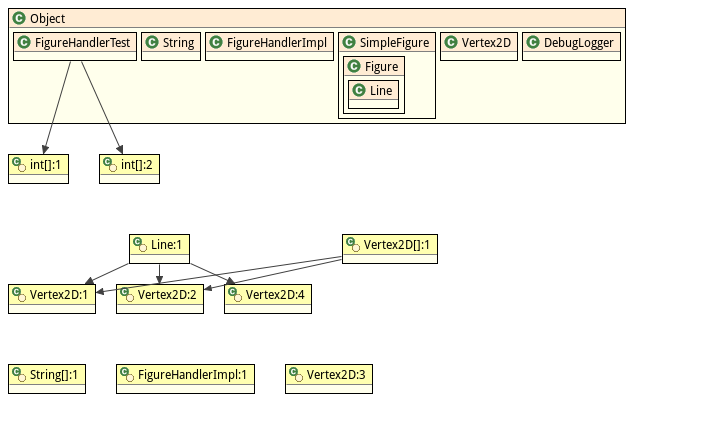
\includegraphics[width=\linewidth]{diagram/figureHandlerTest_Line_Object-Diagram.png}
\caption{Uppgift~3\ref{sec:uppg1b}: Objektdiagram för \texttt{Line}.
\\ (\texttt{diagram/figureHandlerTest\_Line\_Object-Diagram.png})}
\label{fig:obj-line}
\end{figure}

\begin{figure}[ht]
\centering
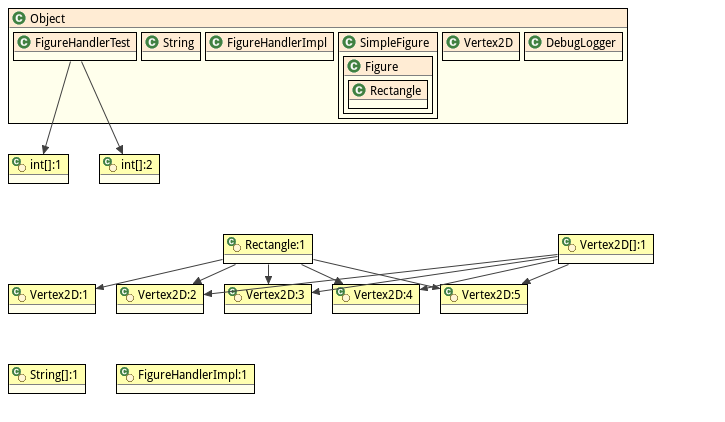
\includegraphics[width=\linewidth]{diagram/figureHandlerTest_Rectangle_Object-Diagram.png}
\caption{Uppgift~3\ref{sec:uppg1b}: Objektdiagram för \texttt{Rectangle}.
\\ (\texttt{diagram/figureHandlerTest\_Rectangle\_Object-Diagram.png})}
\label{fig:obj-rect}
\end{figure}

\subsection{}\label{sec:uppg3b}
\subsubsection*{Frågeställning}
Skriv klasserna som implementerar interfacen i styrnings-API:et enligt figur 7.

\subsubsection*{Lösning}
Se bifogad källkod. Lösningen använder \texttt{StringBuilder} för att
konkatenera resultatet från superklassens \texttt{toString}-metod med klassens
egna data.


\subsection{}\label{sec:uppg3c}
\subsubsection*{Frågeställning}
Diskutera: Varför används typer som \texttt{List<FigureType>} i FigureHandler?
Kan man inte använda bara List? Eller en array?


\subsubsection*{Lösning}
Användningen av en \texttt{List} framför en vanlig array motiveras med att en
array inte kan ändra storlek dynamiskt. Storleken definieras vid skapande av
arrayen och är därefter fixerad. En \texttt{List} har flera användbara
funktioner som saknas för arrays. Genom att skriva något i stil med
\texttt{List<Figure>} specifieras vilken typ av objekt listan kan innehålla.
Det fungerar som en slags felkontroll där kompilatorn ger varningar om ett
inkompatibelt objekt stoppas in.




\end{document}

